\chapter{Signal-quality-based Radio Environment Prediction}
	\label{cha:pred_ho}
	
	Prediction is an often pursued task, because it allows for preparation to upcoming events: weather forecasts allow us to put on the appropriate clothing in the morning, financial forecasts let us invest into the next big stock while it is still cheap, earthquake predictions allows us to move out of harms way in time, etc.
	However, the prediction of events is also complicated, because most of the contexts where it is beneficial to use prediction are also the ones where it is almost impossible to account for all controlling factors, and thus to precisely predict future behavior.
	A famous quote -- likely originating from Niels Bohr -- is fitting here: ``Predictions are hard, especially about the future''.
	A somewhat philosophical question is whether a completely known and enclosed system's behavior could be predicted, as there always seem to be some small variations which we are not able to describe in a systematic way, which could affect even high-level, abstract systems in an unforeseen way.
	Working years on prediction tasks, it seems to me -- and I imagine to many others with similar tasks -- that randomness is ingrained into the universe, and there is no way around it.
	
	% Network planning: https://ieeexplore.ieee.org/abstract/document/7565166
	% Slice maxim: https://ieeexplore.ieee.org/abstract/document/8057230
	% VM migration: https://ieeexplore.ieee.org/abstract/document/7794955
	% Load balancing: https://ieeexplore.ieee.org/abstract/document/8388652
	All is not lost, however, as predictions often don't have to be extremely precise to be useful.
	Furthermore, the farther a prediction is in the future, the less precision is required for usefulness.
	It is important to note: whether or not a prediction is long-term depends on the rate of change in the system that is modeled, and not on the absolute time forward the prediction targets.
	Long-term can mean a few seconds if the changes are very abrupt (such as radio conditions), and conversely, short-term can mean years if the changes are very gradual (such as population density changes).
	Prediction on a long timeframe (years) could be used well in network planning, by using population growth and map data to select locations for new cells \cite{pred_network_planning}.  
	Prediction of medium timeframe changes (hours/minutes) could be used for many orchestration functions, by predicting traffic to maximize the utilization of slices \cite{pred_slicing}, predictively migrating containers/\acp{VM} to follow users \cite{pred_resource_alloc}, or predictively allocating users to balance load between cells \cite{pred_load_balance}.
	In the following work, we discuss predictive handovers, which utilize very short timeframe (seconds) predictions.
	However, because the strength of radio signals can change abruptly (in a few milliseconds), I still consider handover prediction a long-term prediction task.

	Handovers of users between cells are one of the main causes for possible service degradation/interruption, and as such a primary target where cognitive automation could be beneficial.
	In the context of handovers, the basis for better automation is the exact determination -- and in our case prediction -- of points where handovers should be triggered (both in time and space).
	With a precise knowledge of these handover points, handovers can be optimized to simultaneously minimize the number of handovers (and subsequently ping pong handovers) that are triggered, as well as the radio link failures (too early and late handovers) that may result from improper handover settings.
	The minimization of service interruption caused by handovers is critical for \ac{URLLC}, a standout feature of 5G.
	
	This chapter details the work published in the following paper:
	
	\begin{publication}
		Machine-Learning-Based Predictive Handover \\
		\textit{Ahmed Masri, Teemu Veijalainen, Henrik Martikainen, Stephen S. Mwanje, Janne Ali-Tolppa, Márton Kajó} \\
		IM 2021-2021 IFIP/IEEE International Symposium on Integrated Network Management, pp. 1-2. IEEE, 2021.
	\end{publication}

	I contributed to the above research as a \ac{DL} expert, consulting with my colleagues about implementation details and how to best train the deep neural net used for prediction. 
	I also a co-authored and extensively edited the paper, as well as prepared and presented the results at the conference.
	The discussion in this thesis expands on the paper, by providing further details to the inner-workings of the algorithm, as well as showing extended results that were not included in the paper.
	
	\section{Machine-Learning-Based Predictive Handover}
		\label{cha:pred_ho:ml_based_pred_ho}
		
		\subsection{Minimizing Interruption}
		
			A major goal for \ac{5G} networks is to provide \ac{URLLC} \cite{pred_hoinnr}, which could be used, for example, in reliable factory automation, remote control, smart grids, self-driving cars and any critical tasks that rely on close-to-real-time communication. 
			One aspect of the \ac{URLLC} feature is high availability, i.e.: minimization of the times when the communication is interrupted. 
			Handovers are a major cause of interruptions in mobile communications, so for \ac{URLLC} services it is critical that these are minimized.		
			Thus, \ac{URLLC} communication requires a very low \ac{MIT}, defined by the \ac{3GPP} standard as the time during which a user terminal cannot exchange user plane packets as it is handed over from one cell or base station to another \cite{pred_studyonscenarios}.
			
			For a handover event, the \ac{MIT} ($T_{MIT}$) consists of two parts as given by Eq.~\ref{eq:tmit}:
			\begin{equation}\label{eq:tmit}
				T_{MIT} = (1-P_{HOF})*T_{HIT} + P_{HOF}*T_{HOF},
			\end{equation}
			where $T_{HIT}$ is the interruption time during a successful \ac{HO} and the $T_{HOF}$ is the interruption time in case of a \ac{HOF} or a \ac{RLF}.
			A \ac{HOF} occurs, if a \ac{UE} is handed over too early or to a wrong target cell, and a \ac{RLF} occurs when a \ac{HO} is triggered too late or not at all, leading to a lengthy recovery procedure to reconnect to the network \cite{pred_hoinnr}.
			The value $P_{HOF}$ is the probability of either a \ac{HOF} or a \ac{RLF} occurring during a \ac{HO}.
			The total accumulative \ac{MIT} experienced by a \ac{UE} is the product of $T_{MIT}$ and the number of \acp{HO}.
			
			The total $T_{MIT}$ can be reduced by reducing the $P_{HOF}$ or the number of unnecessary \acp{HO}, especially the ping pongs.
			In \ac{LTE} networks, the typical $T_{HIT}$ is reported to be about $50\,ms$ \cite{eutralatency, eutradescription}, while the $T_{HOF}$ ranges from a few hundred milliseconds to several seconds.
			As the $T_{HOF}$ has higher impact on the total $T_{MIT}$ than $T_{HIT}$, it follows that reducing the $P_{HOF}$ will contribute more to reducing the $T_{MIT}$.
			Because the most common cause of a failed handover is a late handover, the usual way of reducing the $P_{HOF}$ is to increase the likeliness of handovers, while keeping in mind that increasing the likeliness of handovers could cause many unnecessarily ping-pongs that may accumulate and increase $T_{MIT}$ just the same.
			Thus, in classical \ac{HO} mechanisms, the reduction of the total $T_{MIT}$ is a balancing game between the number of handovers and handover failures.
			
			\begin{figure}[ht]
				\centering
				\subfloat[Reactive HO]{
					\includegraphics[width=0.48\linewidth]{figures/09_pred_ho/react_pred_ho/reactive_ho.pdf}
					\label{fig:react_pred_ho_reactive_ho}
				}
				\subfloat[Predictive HO]{
					\includegraphics[width=0.48\linewidth]{figures/09_pred_ho/react_pred_ho/predictive_ho.pdf}
					\label{fig:react_pred_ho_predictive_ho}
				}
				\caption[Reactive and predictive handover mechanisms]{Reactive and predictive handover mechanisms.}
				\label{fig:react_pred_ho}
			\end{figure}
		
			Figure~\ref{fig:react_pred_ho_reactive_ho} shows the current reactive \ac{HO} mechanisms.
			Existing adaptive \ac{MRO} solutions (both rule-based automation functions and learning-based functions) select/balance the best handover settings for a given pair of cells, i.e. they optimize the \ac{CIO} and \ac{TTT} settings for a pair of cells.
			The \ac{CIO} parameter (e.g. $1-3\;dB$) acts as a hysteresis value on the received signal quality, delaying handovers until the best cell's signal is \ac{CIO} amounts better than the current serving cell.
			The \ac{TTT} parameter ($0-5000\;ms$) delays \ac{HO} execution, so that the effect of erratic changes is suppressed.
			Both of these parameters are meant to combat sporadic \acp{HO} and ping-pongs, but they can also be the cause of \acp{RLF} if the induced delay is long compared to the rate of change in the radio environment, such as for fast moving cars.
			Furthermore, because a common setting is used over the entire boundary, there may still be areas of poor performance even with optimal parameter values, since the radio conditions are far from uniform across the whole cell border.
			The cell-pair-wise settings are also incapable of accounting for nuances, such as differences in user speed, trajectory across the cell border and temporal changes in the radio propagation environment.
			
			Theoretically -- using perfectly predicted radio conditions -- the balancing game can be escaped, and the $P_{HOF}$ reduced to $0$ while also minimizing the number of handovers (Fig.~\ref{fig:react_pred_ho_predictive_ho}).
			In traditional \acp{HO} implementations, measurements are only logged for specific events, such as logging when two or more handovers happen in a preset timeframe (ping pong \ac{HO}).
			This work studies the possibility of using \ac{ML} to learn the mobility policy based on a constant stream of \ac{UE} measurements and predefined performance objectives.
			This allows the mobility to be dynamically optimized for each \ac{UE} and situation while considering the predicted radio conditions.
			To evaluate this concept, we developed a predictive classifier, which takes \ac{UE} measurements and determines the optimal point in time and the target cell for a \ac{HO}, in order to minimize the total \ac{MIT}.
			The concept was evaluated using simulations in a challenging industrial \ac{5G} network setup.
		
		\subsection{Related Work}

			Several publications have applied \ac{ML} approaches to optimize the performance of \acp{HO} without changing the reactive \ac{HO} regime.
			Most of these works use reinforcement learning techniques, in which a model is trained online by interacting with environment, without the need for prepared training data.
			For example, authors in \cite{rlbasedpredictive} applied a reinforcement learning algorithm called $\epsilon$-greedy Q-learning to learning the optimal \ac{HO} policy, which maximizes the future throughput expected under the locations and velocities of pedestrians.
			Their work depends on slow moving users and a human tracking module, e.g. an RGB-D camera, which makes their reinforcement learning model customized for such non-common scenario.
			However, reinforcement learning techniques have one main drawback, i.e. that the learn-by-experience approach requires a trial and error period, which cannot be tolerated by most real-life environments \cite{rlbasics}.
			For this reason, in this work we focus on unsupervised \ac{ML}, in which training data is collected and an offline model trained, after which an online prediction using the trained model can be executed.
			
			Authors in \cite{predictionbasedcho} proposed an approach toward improving the conditional \ac{HO} technique, by predicting the target cells to be prepared for a possible upcoming \ac{HO}.
			Their results show a promising improvement towards reducing the \ac{MIT}.
			However, the approach was tested with \ac{HO} triggering still using the legacy \ac{LTE} \ac{HO} methods, in a simplistic environment that is not representative of typical 5G \ac{URLLC} conditions.
			
			Authors in \cite{mlbasedho} proposed to assist \acp{HO} in mmWave vehicular networks, by using historical \ac{HO} data and a simple \ac{ML} algorithm to determine the internal relationship between a vehicles’ status information when requesting \acp{HO} and the final \ac{HO} decisions.
			However, their proposal optimized for vehicular networks in a specific scenario, and cannot be generalized for other challenging 5G scenarios.
			
			The work in \cite{exploringtrajectory} focuses on multi-user, multi-step trajectory prediction using the \ac{LSTM} supervised \ac{ML} technique.
			Predicting the user’s future location provides important information towards reducing $T_{HOF}$.
			However, their achieved user location prediction, in the order of dozens of seconds to a few minutes, is too long for industrial environments, e.g. to predict the quick jumps between cells within the few hundreds of milliseconds when user is moving between machines with heavy shadowing effects.
		
		\subsection{Training the Predictor}
		
			\begin{figure}[ht]
				\centering
				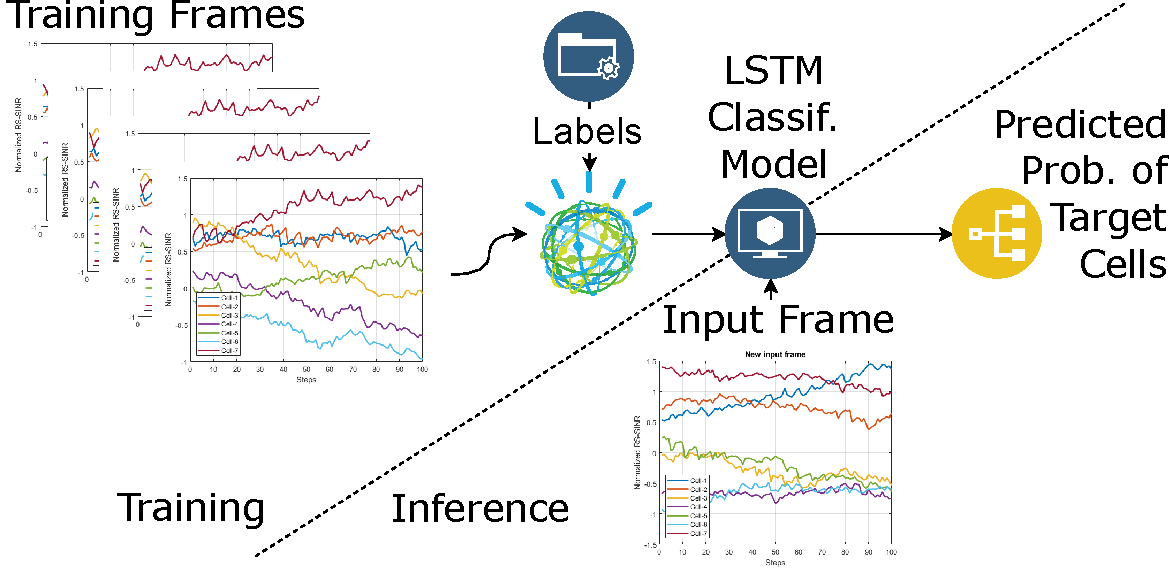
\includegraphics[width=0.64\linewidth]{figures/09_pred_ho/pred_ho_concept/pred_ho_concept.pdf}
				\caption[Predictive handover overview]{Predictive handover overview.}
				\label{fig:pred_ho_concept}
			\end{figure}
			
			The aim of predictive \ac{HO} is to improve mobility performance over state-of-the-art methods (including \ac{MRO}), by learning and optimizing the triggering of \acp{HO} for a particular environment. 
			As shown in Fig.~\ref{fig:pred_ho_concept}, the model is meant to take as input \ac{UE} \ac{SINR} measurements from $K$ specific cells. 
			Theoretically, the model can implicitly finger-print the \ac{SINR} signals -- such as triangulate position -- and learn to predict the probability that a given cell will have the best \ac{SINR} by a future time instance $J$, thus, this fingerprint becomes specific to the geographical area. 
			A \ac{HO} to a cell $C$ is recommended if cell $C$ is not the serving cell and has the highest predicted probability.
			This formulation is a $K$-class classification problem, which we implemented using an \ac{LSTM} neural net.
			
			A key question in classification is how the labels are obtained.
			In our approach, the labels are estimated offline, from recorded \ac{SINR} measurements.
			Each cell is assumed to generate interference for the target candidate cell and the corresponding \ac{SINR} is mapped to a capacity estimate, similar to Shannon's capacity equation, so that the cell with the highest expected capacity over the samples from $t+i$ to $t+M$ is chosen as the best.			
			\ac{SINR} is used to evaluate the spectral efficiency of each cell at a given point in time, where the spectral efficiency is integrated over the labeling window.
			Additional penalties are defined for handovers, such as \acp{UE} receiving zero capacity during the interruption, which ensures to only trigger the necessary \acp{HO} and subsequently limit the ping-pongs.
			Weights are used to balance the trade-off between spectral efficiency and outage from handovers or failures.		
			
			\begin{figure}[ht]
				\centering
				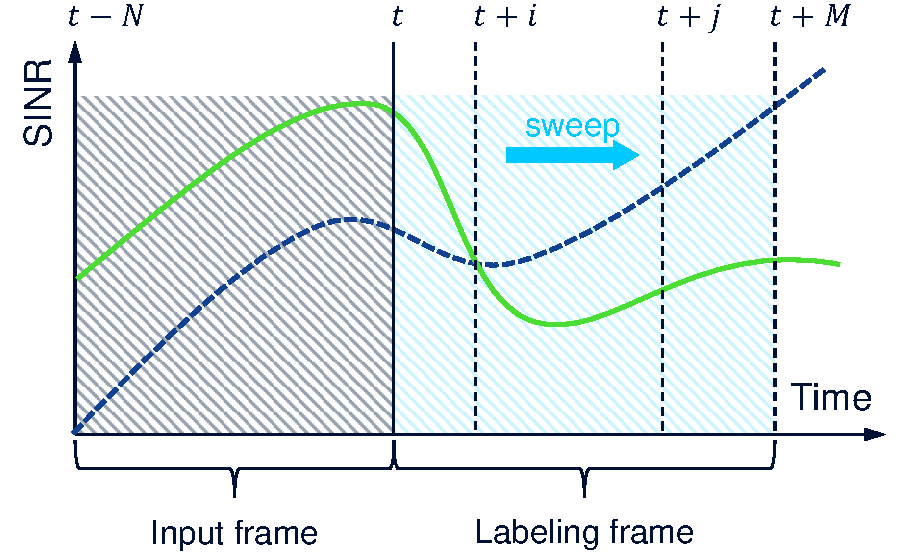
\includegraphics[width=0.5\linewidth]{figures/09_pred_ho/pred_ho_labeling/pred_ho_labeling.pdf}
				\caption[Labeling the training frames for predictive handover]{Labeling of the training frames for the LSTM predictor.}
				\label{fig:pred_ho_labeling}
			\end{figure}
			
			At time $t$, the input for the model is $N$ previous measurements from the $K$ cells, which we call the input frame.
			The label for this input is calculated using the $M$ samples after the input frame, which make up the labeling frame.
			The goodness of a \ac{HO} is estimated for each point $i$ within the $M$ samples by using samples from $i$ to $i+M$ (Fig.~\ref{fig:pred_ho_labeling}).
			Connection to the serving cell is assumed until $t+i$, after which we evaluate -- using the remaining $M-i$ samples -- what would happen if \ac{HO} is triggered at $i$ towards each candidate cell $L$.		
			Since any point $i$ within the $M$ samples could be the optimal \ac{HO} point, the \ac{HO} candidate points $i$ are swept inside the labeling frame until $J$ samples ($J<M$) to determine the best among them.
			Starting with the assumption that point $t$ ($i=0$) is the best \ac{HO} point and towards the serving cell (i.e., no \ac{HO} is necessary), each of the subsequent points are evaluated for each of the candidate target cells, to determine if they provide better connectivity for the user.
			If the newly evaluated point is found to be better than the current best \ac{HO} point, the new point is marked as the current best \ac{HO} point.			
			The evaluation of \ac{HO} candidates continues until $i$ reaches $J$, at which point the best target and time point are chosen as \ac{HO} label for the input at time $t$.
			If no cell is found to be better than the serving cell, we repeat the process by incrementing $t$ by one step.
			Otherwise, the process continues at the obtained \ac{HO} point with the new serving cell.		
		
		\subsection{Filtering Classification Decisions using a Dynamic Threshold}
		
			During the online operational phase, classification inference in cell $A$ is performed at each time step but \ac{HO} is only triggered -- say to cell $B$ -- when the output of the classifier changes between time steps, in this case from cell-$A$ to cell-$B$.
			As in any classification task, precision and recall, and their translated costs are important performance metrics.
			The cost of a false negative -- a handover not triggered in time -- is a \ac{RLF}, from which the recovery can take $10\times$ or $100\times$ longer than the interruption caused by a \ac{HO}.
			However, the cost of false positives -- wrong timing of the \ac{HO} and/or \ac{HO} to the wrong cell -- can also be many times that of a successful \ac{HO}.			
			An unnecessary \ac{HO} may generate e.g. an \ac{RLF} if \ac{HO} is triggered towards a weak cell, or ping-pong if \ac{HO} is triggered towards sub-optimal cell, after which the user is handed back to the optimal cell.
			
			The typical way of controlling for erratic inference is to add a threshold to the output -- after the softmax layer -- acting as a confidence minimum, which the classifier has to reach before a handover is triggered.
			We have devised a method, called \ac{DCT}, which can dynamically adjust this threshold during runtime to balance between false positive and false negative \ac{HO} triggers.			
			The \ac{DCT} adjustment algorithm can be seen on Alg.~\ref{alg:dct}, where $RSSINR_{serv}$ is an $n$-steps history of the serving cell's measured \ac{RSSINR}, and $P_{max}$ is the \ac{ML} model’s max prediction output probability of target different than serving cell.
			$EMA()$ is the exponential moving average function, $RSSINR_{serv}(end)$ is the instantaneous value of the current time step of the serving cell's measured \ac{RSSINR}, $Q_{out}$ is a threshold below which the user is unable to communicate and $DCT_{max}$ and $DCT_{min}$ are the max and min values of \ac{DCT}, respectively.
			$Ref_{max}$ and $Ref_{min}$ are maximum and minimum $SINR$ budgets ($\Delta_2$), outside of which $DCT$ is again restricted to its max and min values.
			Finally, $S_{up}$ and $S_{down}$ are the \ac{DCT} increment up and decrement down step sizes, respectively.		
			The goal of \ac{DCT} is to filter out many of the inaccuracies and noise of the classifier.
			The necessity of using \ac{DCT} will become apparent shortly, in the next section.
		
			\begin{algorithm}[ht]
				\SetAlgoLined
				
				\KwIn{$RSSINR_{serv}$ and $P_{max}$, parameters $S_{up}$ and $S_{down}$}
				\KwOut{Decision: HO (target cell ID) or No-HO}
				$\Delta_1 = EMA(SINR_{serv}) - Q_{out}$\;
				$\Delta_2 = SINR_{serv}(end) - Q_{out}$\;
				\uIf{$\Delta_2 > Ref_{max}$}{
					$DCT = DCT_{max}$\;
				}
				\uElseIf{$\Delta_2 < Ref_{min}$}{
					{$DCT = DCT_{min}$\;}
				}
				\Else{
					\uIf{$\Delta_2 >\Delta_1$}{	
						$DCT =
						\begin{cases}
							DCT + S_{up}\;\; if & DCT + S_{up} \leq DCT_{max}\\
							DCT_{max}\;\; otherwise
						\end{cases}
						$\;
					}
					\Else{
						$DCT =
						\begin{cases}
							DCT - S_{down}\;\; if & DCT - S_{down} \geq DCT_{min}\\
							DCT_{min}\;\; otherwise
						\end{cases}
						$\;       
					} 
				}
				\uIf{$P_{max} \geq DCT$}{ 
					Trigger HO toward predicted target with $P_{max}$\;
				}
				\Else{ 
					No-HO\;
				}
		
				\caption[DCT]{The DCT algorithm.}
				\label{alg:dct}			
			\end{algorithm}
		
		\subsection{Evaluation Environment and Scenario}
		
			Our goal was to evaluate the performance of the predictive \ac{HO} model both with and without the classification threshold (\ac{DCT}) and to compare that performance to the legacy solutions: the baseline with A3 triggering and when applying \ac{MRO}.
			Our study focused on \ac{URLLC} services, requiring that an industrial environment is considered, which we simulated using a proprietary network simulator.
			The network and its processes were simulated by a MATLAB-based simulator, in which a detailed 5G-like radio environment simulating a factory scenario is implemented.
			The \ac{ML} algorithm was implemented in Python.
			
			\begin{figure}[ht]
				\centering
				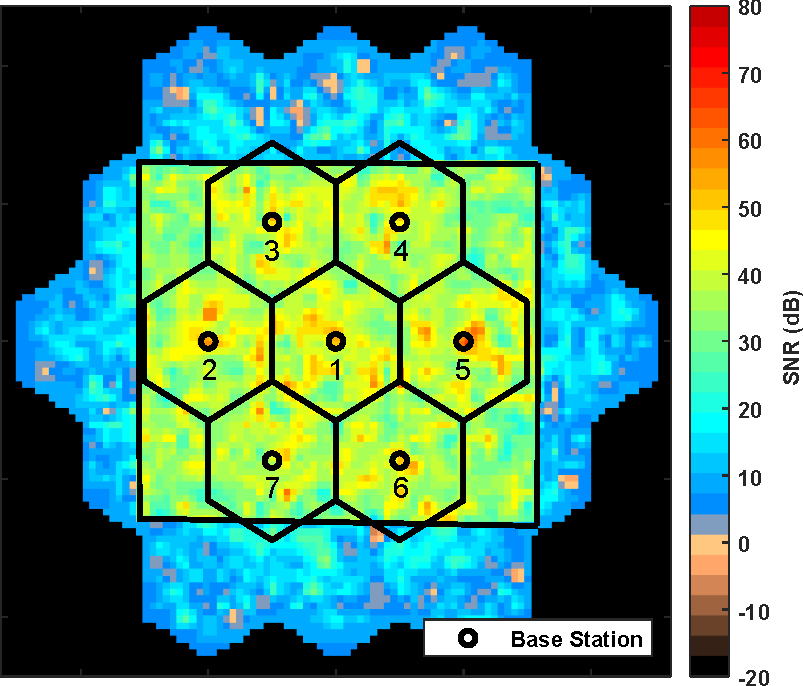
\includegraphics[width=0.6\linewidth]{figures/09_pred_ho/pred_ho_snr_map/pred_ho_snr_map.pdf}
				\caption[SINR map of the simulated scenario in the predictive handover evaluation]{SINR map of the factory environment.}
				\label{fig:snr_map}
			\end{figure}
			
			The simulation considered a radio network in a factory having $M$ micro cells with an inter-site distance of $50\;m$ and $N$ mobile users.
			The factory covered $22500\;m^2$ with surrounding walls limiting the users’ mobility to the factory dimensions, as shown in Fig.~\ref{fig:snr_map}.
			For simplicity, the walls had no reflection effects on signaling, but emulated the internal factory structure, an environment with obstacles and heavy clutter, with path-loss given by Eq.~\ref{eq:path_loss}:
			\begin{equation}
				\label{eq:path_loss}
				PL = PL_0 + 10n\times log_{10}(\dfrac{d}{d_0}) + S,
			\end{equation}
			where $PL_0=80.84\:dBm$ is the free space path loss at reference distance $d_0=15\;m$.
			The path loss exponent $n=1.69$ and the shadowing $S$ is a Gaussian-distributed random variable with zero mean and standard deviation, $\sigma=6.62\;dB$.
			The shadowing correlation and correlation distances were set to $0.5\;m$ and $5\;m$ respectively.
		
			The operating frequency was set to $2.4\;GHz$, and the cells’ transmission power was set to $30\;dBm$ for the whole transmission bandwidth of $100\;MHz$.
			Worth noting from the factory’s \ac{SINR} distribution in Fig.~\ref{fig:snr_map} is that the scenario was not limited by noise, as we targeted an interference limited system.	
			For the \ac{RSSINR}, the \ac{RSRP} values were assumed to be representative on the full bandwidth and correspondingly could be used to calculate full interference.
			For each user $u \in U$ in cell $k \in K$, the received \ac{RSRP} from cell $q$, given as $RSRP_(u,q|k)$, was used to calculate the $RSSINR_(u,q|k)$ in the following way:
			\begin{equation}\label{eq:rs_sinr}
				RSSINR_(u,q|k) = \dfrac{RSRP_(u,q|k)}{\sum_{l\ne{q}}^{K}RSRP_(u,l|k)},\,\forall\,{q\,in\,K}
			\end{equation}
			For traffic, a full buffer traffic model was used, i.e., users always have data to transmit as long they are in connected state.
			The users moved in straight lines (starting in a random direction), and bounced off walls. 
		
			Whenever a \ac{HO} was triggered, it was followed by a prediction break period of $5$ time steps (equivalent to $50\;ms$), within which the \ac{HO} was assumed to be executed and the model was allowed time to prepare for the new cell.
			Correspondingly, no new predictions were undertaken in this timeframe.
			Other details on the simulation scenario are summarized by Tab.~\ref{tab:pred_ho_sim_params}.
			
			\begin{table}[h]
				\renewcommand*{\arraystretch}{1.2}
				\centering
				\begin{tabular}{l|r c l|r}			
					Parameter 							& Value	&	& Parameter						& Value		\\
					\cline{1-2}\cline{4-5}
					A3 \ac{TTT} [ms]					& $200$	&	& $Q_{out}$ [db]				& $-8$		\\
					L3 filtering time constant [ms]		& $50$	&	& $T_{HIT}$ [ms]				& $50$		\\
					Default A3 offset [db]				& $3$	&	& $T_{HOF}$ [ms]				& $600$		\\
					Simulation time [s]					& $100$	&	& Training data frame size		& $7$x$100$	\\
					\ac{UE} speed [km/h]				& $12$	&	& Training data size [frames]	& $4.4$x$10^6$	\\
					Measurement sampling period [ms]	& $10$	&	& Trained model accuracy		& $98\%$		\\
				\end{tabular} 
				\caption[Parameters of the simulation in the predictive handover evaluation]{Radio, ML and simulation parameters for the evaluation of the predictive handover concept.}
				\label{tab:pred_ho_sim_params}
			\end{table}
		
		\subsection{Evaluation Results}
		
			The evaluation assessed the performance of our \ac{ML}-based predictive \ac{HO} against the baseline with A3 event \ac{HO} triggering and a finely tuned and converged \ac{MRO} \cite{mrobeyonddoppler}, comparing the number of handovers triggered, and the subsequent total outage achieved by the algorithms algorithms.
			The total outage is derived as the product of count for the specific \ac{HO} event and the respective $T_{MIT}$.
			
			Figure~\ref{fig:cell_edge} shows an illustrative example of predictive \ac{HO} with and without the classification threshold in response to changes in the signal of the serving cell.
			Initially, cell~$4$ is the serving cell but, as seen in Fig.~\ref{fig:cell_edge_rssinr}, both cells~$4$ and~$5$ have almost equal \ac{SINR} values, indicating that the user may be moving along the cell border.
			In Fig.~\ref{fig:cell_edge_nodct}, we see that the predictive \ac{HO} solution becomes indecisive about the optimal cell and triggers multiple \acp{HO} between the two cells.
			Applying the classification threshold (\ac{DCT}) with a higher threshold value, as shown in Fig.~\ref{fig:cell_edge_dct}, guides the model to only trigger \ac{HO} when another cell is predicted to be better than the serving cell with a significant confidence.
			This reduces the number of unnecessary \acp{HO}, so that all the ping-pongs between cells~$4$ and~$5$ are eliminated.
			
			\begin{figure}[!ht]
				\centering
				\subfloat[Measured RSSINR]{
					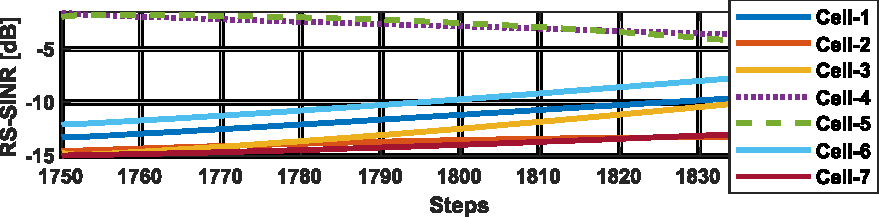
\includegraphics[width=0.8\linewidth]{figures/09_pred_ho/cell_edge/cell_edge_rssinr.pdf}
					\label{fig:cell_edge_rssinr}
				} \\
				\subfloat[Without DCT]{
					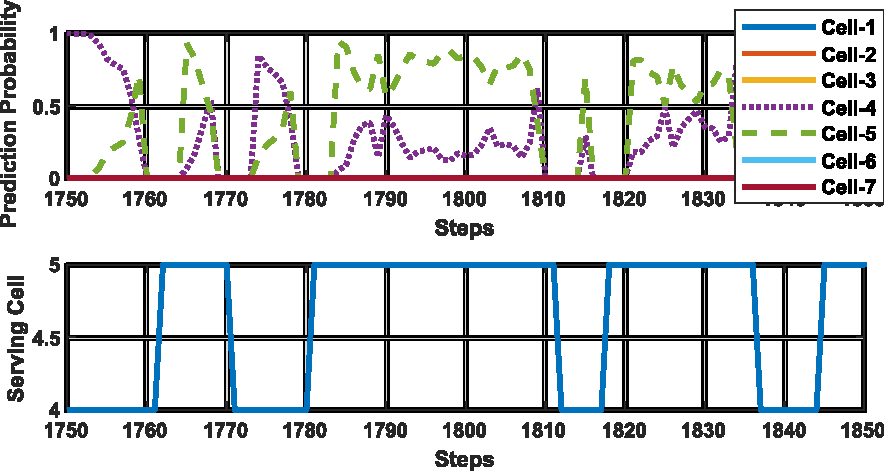
\includegraphics[width=0.8\linewidth]{figures/09_pred_ho/cell_edge/cell_edge_nodct.pdf}
					\label{fig:cell_edge_nodct}
				} \\
				\subfloat[With DCT]{
					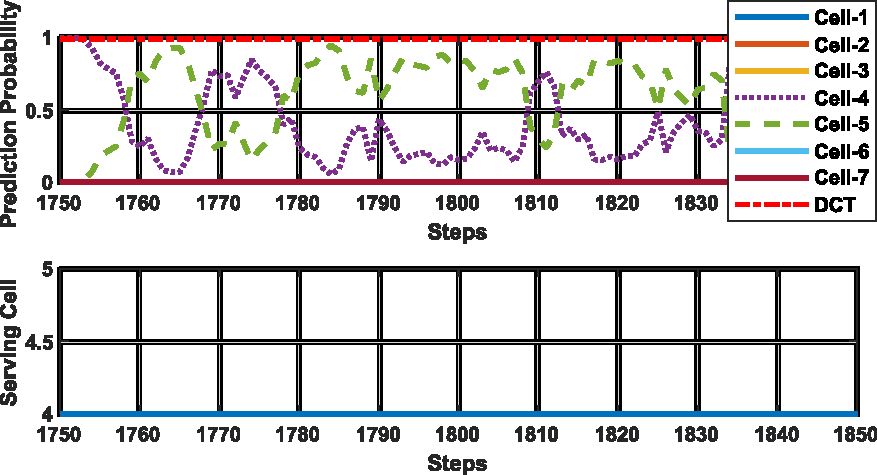
\includegraphics[width=0.8\linewidth]{figures/09_pred_ho/cell_edge/cell_edge_dct.pdf}
					\label{fig:cell_edge_dct}
				}
				\caption[Predictive handover example]{Example of predictive handover for a user moving along the edge of cells~$4$ and~$5$, with and without DCT.}
				\label{fig:cell_edge}
			\end{figure}
		
			Figure~\ref{fig:pred_ho_bars} presents the statistical comparison between the \ac{ML} and non-ML-based solutions.
			Based on the total outage, we observe that the predictive \ac{HO} with \ac{DCT} outperforms all other techniques, including the finely tuned and converged \ac{MRO}.
			Figure~\ref{fig:pred_ho_bars_outage} shows a big reduction in outage, which is a result of a significant reduction in the number of \acp{RLF} (leading to reduced $T_{HOF}$), from $8$ RLF/min in the baseline and $2$ RLF/min for the \ac{MRO} algorithm to less than $0.5$ RLF/min when using the \ac{ML}-based predicted \ac{HO}.
			For the default \ac{ML}-based predictive algorithm, the reduction in \ac{RLF}-triggered outage comes with increased outage due to unnecessary \acp{HO}, which the \ac{DCT} resolves by reducing the per-minute number of \acp{HO} triggered (Fig.~\ref{fig:pred_ho_bars_ho}).

			\begin{figure}[!ht]
				\centering
				\subfloat[Outages]{
					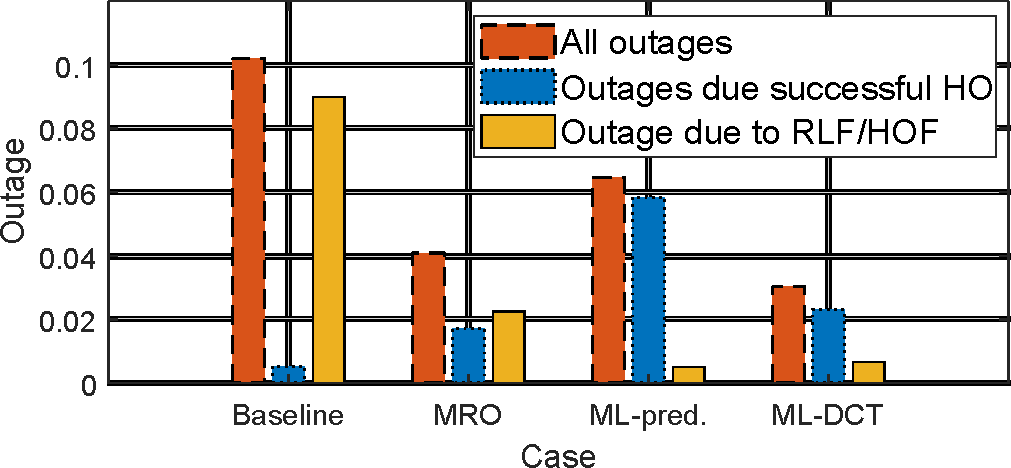
\includegraphics[width=0.6\linewidth]{figures/09_pred_ho/pred_ho_bars/pred_ho_bars_outage.pdf}
					\label{fig:pred_ho_bars_outage}
				} \\			
				\subfloat[Handovers]{
					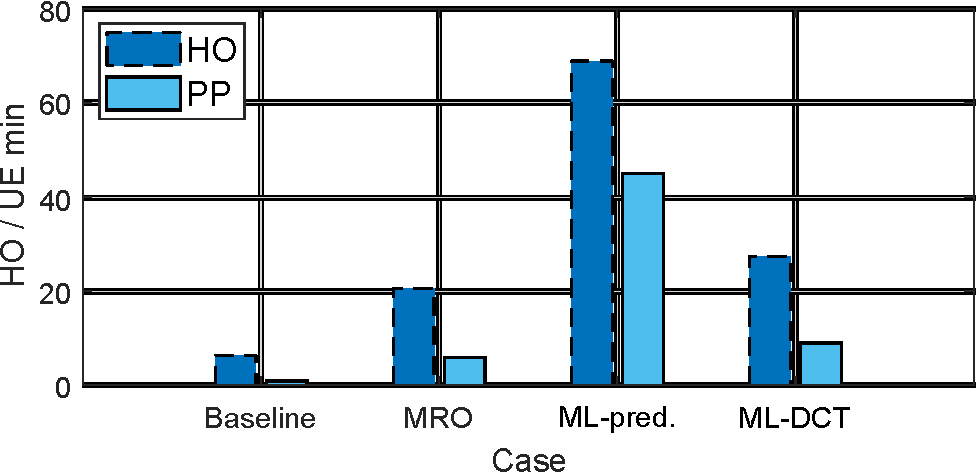
\includegraphics[width=0.6\linewidth]{figures/09_pred_ho/pred_ho_bars/pred_ho_bars_ho.pdf}
					\label{fig:pred_ho_bars_ho}
				}
				\caption[Predictive handover evaluation results]{Comparisons between baseline, MRO and ML-DCT handover statistics.}
				\label{fig:pred_ho_bars}
			\end{figure}
		
		\subsection{Conclusion and Critique}
			\label{cha:pred_ho:sec:crit}
		
			This chapter investigated an \ac{ML}-based \ac{HO} method, which utilizes deep learning to predictively trigger handovers, in order to minimize service interruption time.
			The predictive handover method has been evaluated in a complex industrial environment, where it showed a reduction in the number of radio link failures and total outage from \ac{UE} mobility compared to traditional \ac{HO} triggering as well as the finely-tuned \ac{MRO}.
			While the evaluation results show a very promising performance increase, I think there are a few aspects of the algorithm that could be criticized, and should be improved before it is viable for a real deployment.
			
			The first of these aspects is the algorithm's heavy dependence on \ac{DCT}, without which the performance is sub-par compared to the traditional, non-\ac{DL}-based \ac{MRO} optimization (Fig.~\ref{fig:pred_ho_bars}).
			To me, this, and the erratic behavior depicted in Fig.~\ref{fig:cell_edge_nodct} when not employing \ac{DCT} signals that the prediction is not as dependable as it perhaps should be.
			I suspect that \ac{DCT} could have been omitted with a better predictor, as it stands in this evaluation, \ac{DCT} is a necessary ``crutch'' for an improperly working predictor.
			It would have been interesting to see just how much performance \ac{DCT} adds to the system if the prediction is better, however, this evaluation is not so straight-forward, because the output of the predictor is a categorical cell-probability.
			With a continuous (regression) prediction task, the prediction could be linearly mixed with the true future, thus evaluating \ac{DCT}'s value without actually having to implement a perfect predictor.
			This also leads to the next problematic aspect.
			
			The second aspect is the categorical prediction that is required form the predictor, where seemingly tiny changes in the input \ac{RSSINR} values warrant sudden, complete changes in the output.
			In my experience, such tasks are not well-fitting for neural nets, because even though neural nets employ many layers with plenty of nonlinearities to be able to approximate such functions, they still behave similarly to signal amplifiers: if neural nets learn to approximate steep changes in the output for certain small input changes, they will also map similarly large output changes to other small input changes, where they are not necessarily needed.
			In this analogue, the neural net learns to model an amplifier with a high rate of amplification.
			This also explains the erratic predictor output, and the need for \ac{DCT}.
			Overall, I think a differently formulated prediction task would fit neural nets better, where small changes in the input correspond to similarly small changes in the output.
			
			The third problematic aspect is the required inputs for the predictor: the \ac{RSRP} measurements are required from all cells at all times for each user.
			This is not a realistic scenario, because users often don't ``see'' all cells, i.e.: some cells' signals are such a low power that they vanish in the interference or background noise.
			This problem becomes more severe the larger the scenario is, or the more cells it includes.
			Thus, either a model needs to be developed which can handle missing inputs -- which is generally a problem for neural nets, a topic which is the focus of Part~\ref{part:confidence} -- or different measurements should be used, which are always accessible.
			Furthermore, the noisy nature of radio measurements -- such as \ac{RSRP} -- also contribute to the erratic predictions, where other inputs with less variance could prove to be smoother, and thus easier to predict.
			
			All of these aspects were taken into account when we researched mobility-based radio prediction, the topic of the next chapter.
